\section{Введение}
Лабораторная работа по курсу \textquotedblleft{}Алгоритмы и анализ сложности\textquotedblright{}. Алгоритм Грэхема: с использованием быстрой сортировки и с использованием сортировки, основанной на АВЛ-дереве.

\subsection{Постановка задачи}

\noindent \textbf{Постановка задачи построения выпуклой оболочки}\\
\indent Для точек $a_1, ..., a_n$, где $n\geq1$, $a_i=(a_{i,1},a_{i,2})\in R^2$ при $i=1,...,n$, указать вершины $b_1,...,b_m$ выпуклой оболочки $Conv(a_1,...,a_n)$ в порядке их встречи при движении по ее границе. В общем случае $Conv(a_1,...,a_n)$ является многоугольником, а в вырожденных случаях может получиться отрезок или точка. В случае отрезка выходом алгоритма, решающего поставленную задачу, должны быть две точки, являющиеся его концами, а в случае точки -- сама эта точка.

\begin{figure}[h]
	\centering
	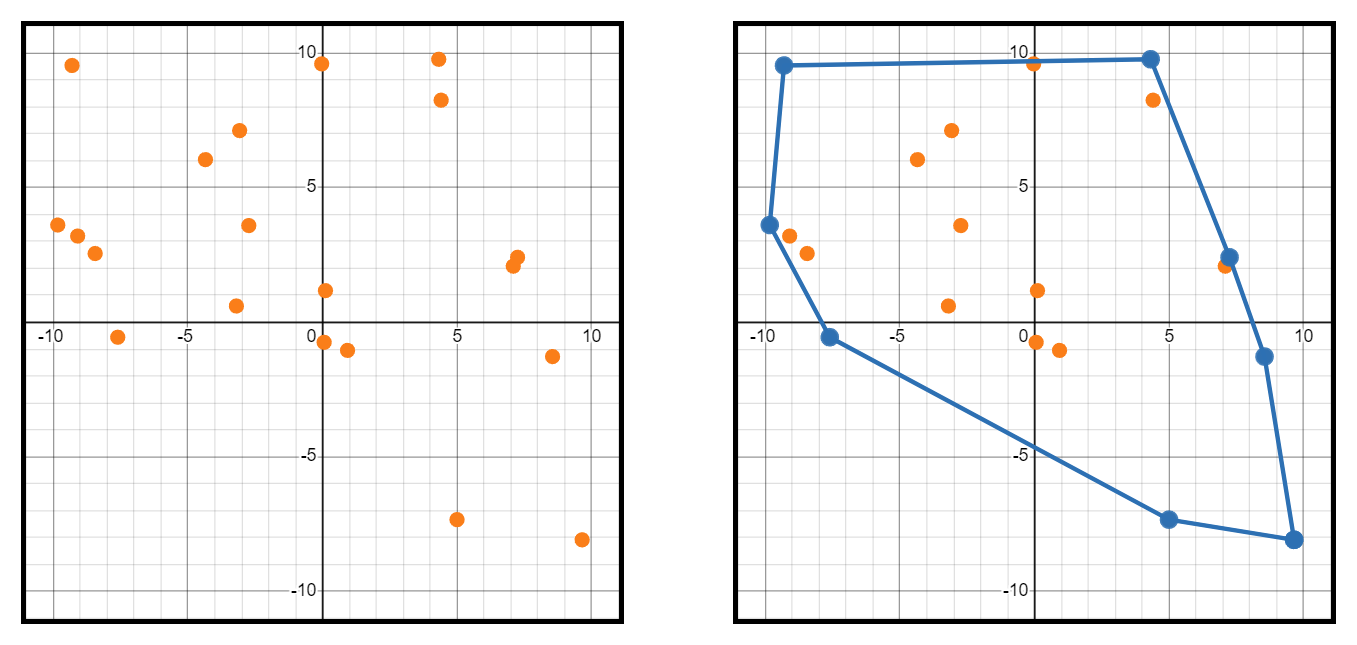
\includegraphics[width=\textwidth]{Images/convex_hull_example.png}
	\caption{Пример выпуклой оболочки точек. Граница выпуклой оболочки и точки, являющиеся её вершинами, обозначены синим. Для примера взяты точки из файлов \textsl{/Program1/Input.txt} и \textsl{/Program1/Output.txt}}
	\label{fig:convex_hull_example}
\end{figure}

\noindent \textbf{Цель лабораторной работы}\\
\indent Сравнение и анализ двух алгоритмов, решающих задачу: алгоритм Грэхема с использованием быстрой сортировки, алгоритм Грэхема с использованием сортировки, основанной на АВЛ-дереве.

\newpage

\noindent \textbf{План лабораторной работы}:
\begin{enumerate}
	\item{($Program1$) Первая программа: чтение из файла входных данных, на выходе - файл с результатами работы алгоритма и временем работы.}
	\item{($Program2$) Вторая программа: проведение экспериментов над реализованными алгоритмами:
		\begin{itemize}
			\item[--]{Генератор тестов для проведения экспериментов, в котором можно выбрать:
				\begin{itemize}
					\item[+]{Кол-во точек $n$ в исходном массиве $a$.}
					\item[+]{Натуральные числа $q$ и $w$.}
					\item[+]{Режимы: ($A$) псевдослучайные точки в прямоугольнике со сторонами $q$ и $w$, ($B$) псевдослучайные точки на границе (на сторонах) этого прямоугольника.}
			\end{itemize}}
			\item[--]{Провести следующие эксперименты:
				\begin{itemize}
					\item[+]{Эксперимент 1 ($E1$) $q = 10^6, w = 10^6$, $n = 1, ..., 10^6+1$ с шагом $10^4$ в режимах ($A$) и ($B$). Построить графики $T_A(n)$ и $T_B(n)$.}
					\item[+]{Эксперимент 2 ($E2$) $q = w = 0, ..., 10^6$ с шагом $10^4$, $n = 10^6$ в режимах ($A$) и ($B$). Построить графики $T_A(q)$ и $T_B(q)$.}
			\end{itemize}}
		\end{itemize}
	}
	\item{Сформулировать и обосновать вывод о том, в каких случаях целесообразно применять какой из алгоритмов.}
\end{enumerate}

\newpage

\subsection{Структура проекта}
\noindent \textbf{Program1}: Реализация первой программы ($Program1$):\\
Файлы: \textsl{/Program1/main.cpp}\\
\noindent \textbf{Program2}: Реализация второй программы ($Program2$):\\
Файлы: \textsl{/Program2/main.cpp}\\
\noindent \textbf{GrahamScan}: Реализация алгоритма Грэхема:\\
Файлы: \textsl{/GrahamScan/GrahamScan.h}, \textsl{/GrahamScan/GrahamScan.cpp}\\
\noindent \textbf{QuickSort}: Реализация быстрой сортировки:\\
Файлы: \textsl{/QuickSort/QuickSort.h}, \textsl{/QuickSort/QuickSort.cpp}\\
\noindent \textbf{AVLTree}: Реализация АВЛ-дерева:\\
Файлы: \textsl{/AVLTree/AVLTree.h}, \textsl{/AVLTree/AVLTree.cpp}\\
\noindent \textbf{Utils}: Общие функции и классы, необходимые для реализации алгоритмов:\\
Файлы: \textsl{/Utils/Utils.h}, \textsl{/Utils/Utils.cpp}\\
\noindent \textbf{Utils\_IO}: Функции для ввода и вывода:\\
Файлы: \textsl{/Utils/Utils\_IO.h}, \textsl{/Utils/Utils\_IO.cpp}\\
\noindent \textbf{Utils\_TestGen}: Функции для генерации тестов:\\
Файлы: \textsl{/Utils/Utils\_TestGen.h}, \textsl{/Utils/Utils\_TestGen.cpp}\\

\begin{figure}[h]
	\centering
	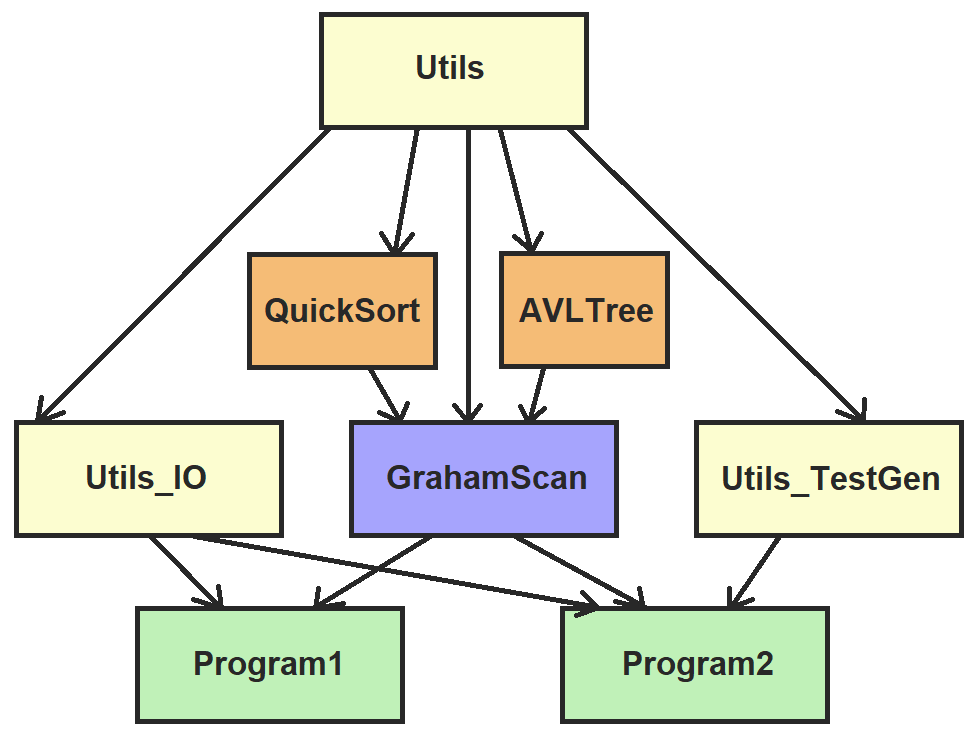
\includegraphics[width=0.7\textwidth]{Images/project_structure.png}
	\caption{Граф зависимостей}
	\label{fig:project_structure}
\end{figure}

\noindent Репозиторий проекта на Github:\\ \url{https://github.com/Damlrca/AiAS_GrahamScan}

\newpage
